\documentclass[border=3pt]{standalone}
% Preâmbulo compartilhado pelos diagramas TikZ da aula 11 (Localização por Grade e Monte Carlo)
\usepackage[T1]{fontenc}
\usepackage[utf8]{inputenc}
\usepackage{lmodern}
\usepackage{amsmath}
\usepackage{xcolor}
\usepackage{tikz}
\usetikzlibrary{arrows.meta,angles,quotes,decorations.pathmorphing,calc,
                positioning,shapes.geometric,shapes.misc,backgrounds,fit,
                math}

% Paleta (mesma dos SVGs originais)
\definecolor{dblue}{HTML}{2A5B8C}
\definecolor{dorange}{HTML}{B3541E}
\definecolor{dgreen}{HTML}{4A7C59}
\definecolor{dred}{HTML}{9C4B4B}
\definecolor{dcream}{HTML}{F4F1EA}
\definecolor{dshade}{HTML}{DDD7C9}

% Função gaussiana (não normalizada por padrão de escala visual)
\pgfmathdeclarefunction{gauss}{3}{%
  \pgfmathparse{1/(#3*sqrt(2*pi))*exp(-((#1-#2)^2)/(2*#3^2))}%
}

% Estilos comuns (prefixo d... para não colidir com chaves internas do pgf)
\tikzset{
  >={Stealth[length=2mm]},
  dguide/.style={gray!55, dashed, line width=0.4pt},
  daxis/.style={gray!60, line width=0.7pt, ->},
  dbody/.style={fill=black!3, draw=black!80, line width=1pt},
  dacc/.style={draw=dblue, line width=1pt},
  dlbl/.style={black!55, font=\small},
  dsub/.style={black!45, font=\footnotesize},
  dstate/.style={circle, draw=black!80, fill=dcream, line width=1pt,
                 minimum size=17mm, font=\large, inner sep=1pt},
  dobs/.style={circle, draw=black!80, fill=dshade, line width=1pt,
               minimum size=14mm, font=\large, inner sep=1pt},
  dbox/.style={rounded corners=2pt, draw=black!80, fill=dcream, line width=1pt,
               align=center, inner sep=6pt},
  dop/.style={circle, draw=black!80, fill=white, line width=1pt,
              minimum size=6mm, inner sep=0pt, font=\small},
  dtrans/.style={->, dblue, line width=1pt},
  dmeas/.style={->, dorange, line width=1pt},
  dcurve/.style={line width=1pt, dblue},
  dcurveb/.style={line width=1.4pt, dorange},
}

\begin{document}
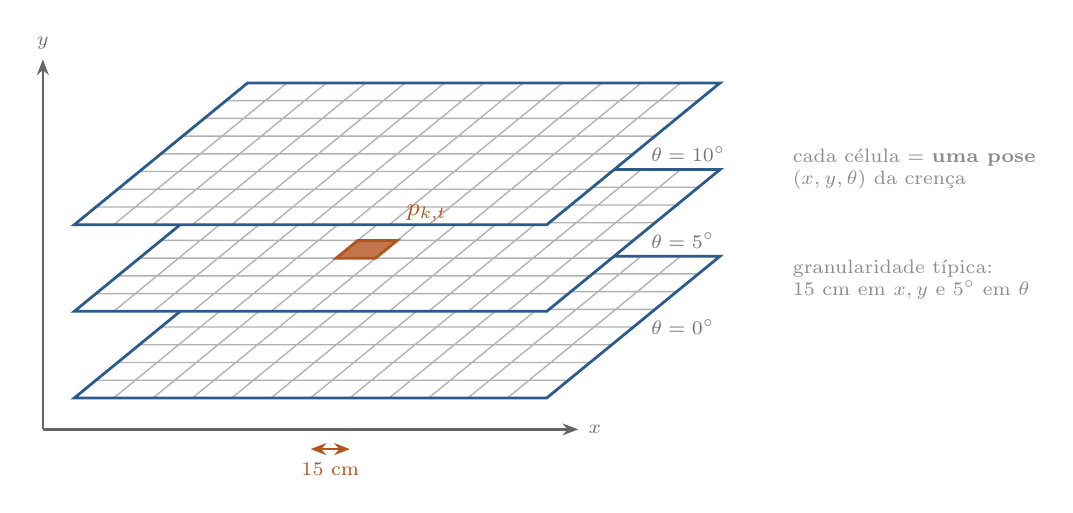
\begin{tikzpicture}[x=1cm,y=1cm]
  \newcommand{\camada}[3]{% desloc-x, desloc-y, rótulo
    \begin{scope}[shift={(#1,#2)}, cm={1,0,0.55,0.45,(0,0)}]
      \fill[white] (0,0) rectangle (6,4);
      \draw[black!30, line width=0.5pt] (0,0) grid[step=0.5] (6,4);
      \draw[dblue, line width=1pt] (0,0) rectangle (6,4);
    \end{scope}
    \node[dlbl, font=\scriptsize, anchor=west] at (#1+7.2,#2+0.9) {#3};
  }
  \camada{0}{0}{$\theta = 0^\circ$}
  \camada{0}{1.1}{$\theta = 5^\circ$}
  \camada{0}{2.2}{$\theta = 10^\circ$}
  % célula destacada na camada do meio
  \begin{scope}[shift={(0,1.1)}, cm={1,0,0.55,0.45,(0,0)}]
    \fill[dorange!80] (2.5,1.5) rectangle (3,2); \draw[dorange, line width=1pt] (2.5,1.5) rectangle (3,2);
  \end{scope}
  \node[dorange, font=\small, anchor=west] at (4.1,2.35) {$p_{k,t}$};
  % eixos
  \draw[->, black!60, line width=0.8pt] (-0.4,-0.4) -- (6.4,-0.4) node[right, dlbl, font=\scriptsize] {$x$};
  \draw[->, black!60, line width=0.8pt] (-0.4,-0.4) -- (-0.4,4.3) node[above, dlbl, font=\scriptsize] {$y$};
  % cotas
  \draw[<->, dorange, line width=0.9pt] (3.0,-0.65) -- (3.5,-0.65);
  \node[dorange, font=\scriptsize, anchor=north] at (3.25,-0.7) {15 cm};
  \node[dsub, font=\scriptsize, align=left, anchor=west] at (9,2.9) {cada célula = \textbf{uma pose}\\ $(x, y, \theta)$ da crença};
  \node[dsub, font=\scriptsize, align=left, anchor=west] at (9,1.5) {granularidade típica:\\ 15 cm em $x, y$ e 5$^\circ$ em $\theta$};
\end{tikzpicture}
\end{document}
